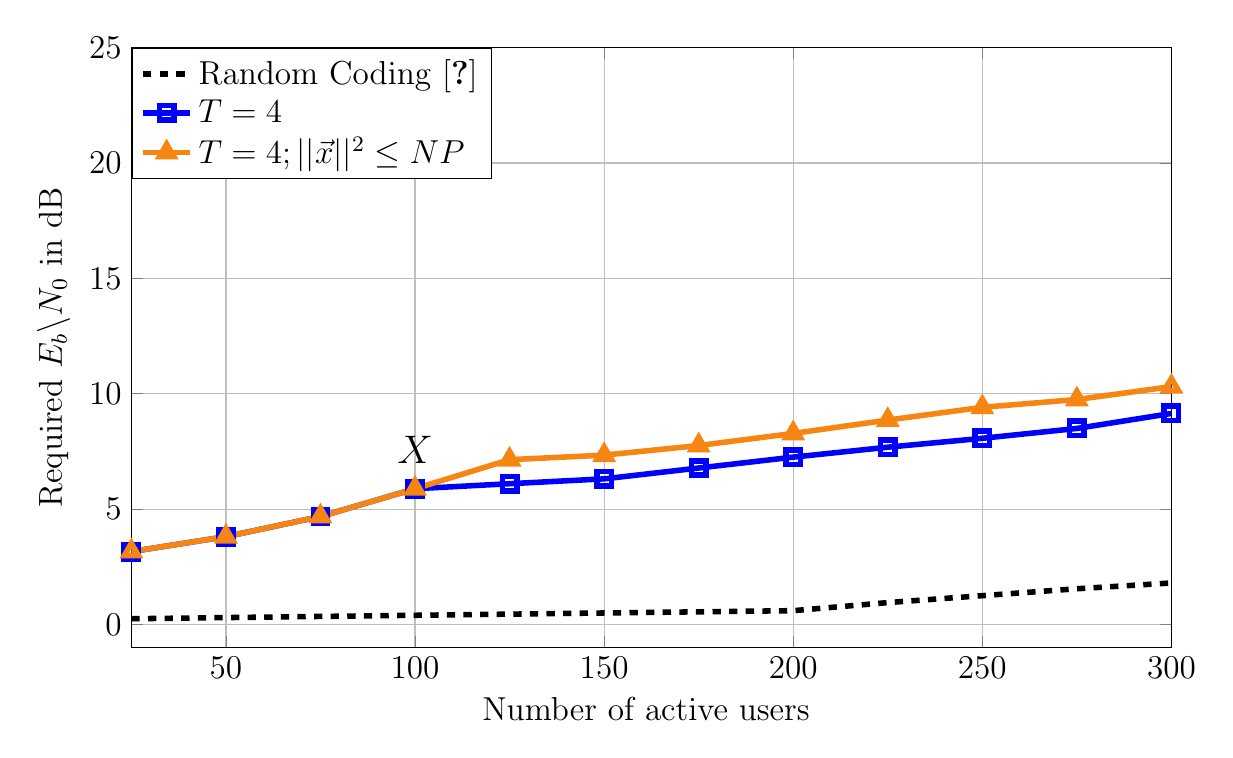
\begin{tikzpicture}
% The SC paramaters for the below set of plots are
% L=16
% w=3.
% So the true rate R is related to design rate R'(=1-dc/dv) as
% 1-R=(L+w-1)*(1-R')/L
\def\fsize{\large}
\pgfplotsset{every y tick label/.append style={font=\fsize}}
\pgfplotsset{every x tick label/.append style={font=\fsize}}

\begin{axis}[%
width=5.2in,
height=3in,
scale only axis,
xmin=25,
xmax=300,
xtick = {50,100,...,300},
xlabel={\fsize{Number of active users $\Ka$}},
ylabel={\fsize{Required $E_b\backslash N_0$ in dB}},
xmajorgrids,
xminorgrids,
ymin=-1,
ymax=25,
ytick = {-5,0,...,30},
yminorticks=true,
ymajorgrids,
yminorgrids,
legend style={at={(0,1)},anchor=north west, draw=black,fill=white,legend cell align=left,font=\fsize}
]

\node[] at (axis cs: 100,7.5696) {\Large $X$};

\addplot [color=black,solid,dashed, line width=2.0pt]
  table[row sep=crcr]{
  25     0.25\\
 50     0.3\\
 75     0.35\\
100     0.4\\
125     0.45\\
150     0.5\\
175    0.55\\
200  0.60\\
225 0.95\\
250 1.25\\
275 1.55\\
300 1.8\\
};
\addlegendentry{Random Coding \cite{polyanskiy2017perspective} };

%\addplot [color=magenta,dotted,line width=2.0pt]
%  table[row sep=crcr]{
%  25   2.26  \\
%  50   2.88  \\
%  75   3.90  \\
% 100   5.03 \\
%  125.0000    5.8798 \\
%  150.0000    7.3954 \\
%  175.0000    8.6199 \\
%  200.0000    9.7328 \\
%  225.0000   11.1761\\
%  250.0000   12.6127\\
%  275.0000   13.3907\\
%  300.0000   14.9116\\
%  };
%\addlegendentry{4-fold ALOHA \cite{ordentlich2017low}};

%\addplot [color=red,solid,mark=diamond,mark size=3.2,line width=2.0pt]
%  table[row sep=crcr]{
%  25   3.5820  \\
%  50   5.2585 \\
%  75   5.8700  \\
%100  6.6738 \\
%125  7.1463 \\
%150  7.9984 \\
%175  8.63 \\
%200  9.55 \\
%225  10.46 \\
%250  11.42 \\
%275 13.4438 \\
%300 14.8439 \\
%};
%\addlegendentry{$T=2$};

\addplot [color=blue,solid,mark=square,mark size=2.6,line width=2.0pt]
  table[row sep=crcr]{
 25 3.1608  \\
 50 3.8064 \\ %lambda=1.0
 75 4.6803\\
100 5.8835\\
125  6.1017 \\
150  6.3117 \\
175  6.7814 \\
200  7.2532 \\
225  7.6838 \\
250  8.0691\\
275  8.4960 \\
300 9.1467 \\
};
\addlegendentry{$T=4$};

\addplot [color=BurntOrange,solid,mark=triangle,mark size=3.0,line width=2.0pt]
  table[row sep=crcr]{
 25 3.1608  \\
 50 3.8064 \\
 75 4.6803\\
100 5.8835\\
125 7.1428\\
150 7.3395\\
175 7.7561\\
200 8.2802 \\
225 8.8590 \\
250 9.4124 \\
275 9.7502\\
300 10.3086\\
 };
\addlegendentry{$T=4;||\vec{x}||^2\leq NP$};



%\addplot [color=blue,dashed,line width=2.0pt]
%  table[row sep=crcr]{
%  25   7.50 \\
%   35   7.30 \\
%  50   8.75 \\
%  100 11.7 \\
%  150 14.50\\
%%175  6.7814 \\
%200  18\\
%%225  7.6838 \\
%250  21\\
%%275  8.4960 \\
%300 23\\
%};
%\addlegendentry{OP-Exact\cite{ordentlich2017low}};

\end{axis}
\end{tikzpicture}


%Old result with error in random_coding_GMAC: used log2 instead of log
%\addplot [color=red,solid,mark=diamond,mark size=4.0]
%  table[row sep=crcr]{
%  25   2.1522  \\
%  50   4.0581\\
%  75   4.5625\\
%100  5.3325 \\
%125    5.4330\\
%150  5.8549 \\
%175  6.3787\\
%200  6.6580 \\
%225  7.9109\\
%250  8.5476\\
%275   9.5476\\
% 300 10.3177\\
%};
%\addlegendentry{T=2};

%\addplot [color=blue,solid,mark=square,mark size=3.0]
%  table[row sep=crcr]{
% 25 2.1178\\
% 50 2.6828\\
% 75 3.1482 \\
%100 3.7733\\
%125 4.6866\\
%150 5.4191\\
%175 5.4495\\
%200 5.6737\\
%225 6.0074\\
%250 6.0881\\
%275 6.9083\\
%300 6.8751\\
%};
%\addlegendentry{T=4};
